%
\documentclass[twocolumn,twoside]{svmultivs_gm} %please do not change this line
\usepackage{graphicx}
%
\title*{Making Where Available to the Community}
%\subtitle{Optional Sub-title on first page}
\titlerunning{Making Where Available}
%
% The contents of \title* are printed on the first page.
% The contents of \subtitle are printed below the title on the
% first page.  This keyword is optional.
% The contents of \titlerunning are printed on the other pages.
% This should be a short version of the title.
%
% Example:
% \title*{Investigation into Radio Frequency Interfence at VLBI Stations}
% \subtitle{A Study of Five Cases}
% \titlerunning{RFI Investigation}
%
\author{Geir Arne Hjelle, Ann-Silje Kirkvik, Michael D\"ahnn, Ingrid Fausk}
\authorrunning{Hjelle et al.} %see comments below
\authoremails{geir.arne.hjelle@kartverket.no,ann-silje.kirkvik@kartverket.no}
\institute{Norwegian Mapping Authority}
%
% \author and \institute keywords:
%
% Each number in \author refers to an institution with which the author is associated.
% The numbers should correspond to numbered institutions in the \institute keyword.
% If all authors are associated with only one institution (the same institution), 
% then the numbers should be omitted from \author and \institute.
% If an author is associated with two or more institutions, multiple numbers may be
% used.
%
% The \institute key word must be a single line.
% Please separate institutions using \\ between each institution.
%
% \authorrunning keyword:
%
% For one author, please use \authorrunning{last_name_of_author}, 
% e.g., \authorrunning{Gordon}
% For two authors, please use \authorrunning{last_name_of_first_author and last_name_of_second_author}
% e.g., \authorrunning{Gordon and MacMillan}
% For three or more authors, please use \authorrunning{last_name_of_first_author et al.}
% e.g., \authorrunning{Gordon et al.}
%
% Examples:
%
% \author{Dirk Behrend}
% \authorrunning{Behrend}
% \author_emails{dirk.behrend-1@nasa.gov}
% \institute{NVI, Inc.}
%
% \author{Karen Baver, Dirk Behrend}
% \authorrunning{Baver and Behrend}
% \author_emails{karen.d.baver@nasa.gov,dirk.behrend-1@nasa.gov}
% \institute{NVI, Inc.}
%
% \author{John Gipson~$^1$, David Eriksson~$^{1,2}$, Dan MacMillan~$^1$}
% \authorrunning{Gipson et al.|
% \institute{1. NVI, Inc.\\ 2. Chalmers University of Technology}
%
\ContactAuthorName{Geir Arne Hjelle}
\ContactAuthorTelephone{+47 93211279}
\ContactAuthorEmail{geir.arne.hjelle@kartverket.no}
%
% \ContactAuthorName, \ContactAuthorTelephone, and \ContactAuthorEmail 
% should be used to identify the preferred contact author.
%
\NumberofInstitutions{1}
\InstitutionPostAddress{1}{N.A}
\InstitutionCountry{1}{N.A}
\InstitutionWebPage{1}{N.A}
%
% Please change \NumberofInstitutions as needed.
% Please add or delete \InstitutionPostAddress, \InstitutionCountry, and
% \InstitutionWebPage as needed.
%
% The keywords \InstitutionPostAddress, \InstiutionCountry, and 
% \InstitutionWebPage are required to let the IVS publications software
% operate.  But the contents of these keywords may be any value for the IVS 
% General Meeting Proceedings. So the content may be kept as N.A.
% or filled in.
%
%
\newcommand{\code}[1]{{\footnotesize\texttt{#1}}}
\newcommand{\where}{\textsf{Where}}
\newcommand{\there}{\textsf{There}}
\newcommand{\midgard}{\textsf{Midgard}}
%
\begin{document}  %please do not change this line
%
\maketitle       %please do not change this line
%
\abstract{The Norwegian Mapping Authority is an associated analysis center within the IVS, and is currently preparing to contribute VLBI analyses to the IVS with its new \where\ software. The software is being made available to the geodetic community under an open source MIT license. You can download \where\ from GitHub and try it for yourself. \where\ is written in Python, and comes with a graphical tool called \there\ that can be used to analyse results from \where\ and edit sessions. Furthermore, a geodetic Python library called \midgard\ is made available. This library contains components of \where\ that are useful in a wider setting. If you are doing any geodetic data analysis in Python, \midgard\ might be useful to you.}
%
\keywords{VLBI, Software, Python, Open source}
%
%  Please fill in one or more keywords in \keywords{}.  
%  One to five keywords is the suggested range.
%
\section{Introduction}
%
The Norwegian Mapping Authority (NMA) has been developing a new software for geodetic analysis the over last years~\cite{kirkvik2017a,kirkvik2017b}. That software is called \where, and is currently being used in NMA's bid for becoming an operational analysis center within the International VLBI Service for Geodesy and Astrometry (IVS)~\cite{kirkvik2018}. In addition NMA has made \where\ available to the community as open source software~\cite{where_joss} under the MIT license.

The \where\ software is currently able to analyse single VLBI sessions, where ambiguities have already been resolved (level 4 databases). There are plans to extend the capabilities of the software going forward, including preliminary support for SLR and GNSS analyses.

The background for why NMA has developed a new software, which models are available, as well as early benchmarks and results are covered in~\cite{kirkvik2017b} and~\cite{kirkvik2018}. This note will focus more on how you can obtain and use the software yourself.
%
\section{Overview of \where}
%
The \where\ software is mainly written in Python\footnote{\url{www.python.org}}. It is cross platform and can run on Linux, macOS, and Windows. \where\ is available for download at

\begin{center}
\footnotesize\texttt{\url{kartverket.github.io/where/}} 
\end{center}

\where\ can do different kinds of analyses. Each kind of analysis is defined as a pipeline consisting of separate steps or stages. Currently, only the VLBI pipeline is publicly available, but work on other pipelines based on SLR and GNSS is underway.

\begin{figure}[htb!]
  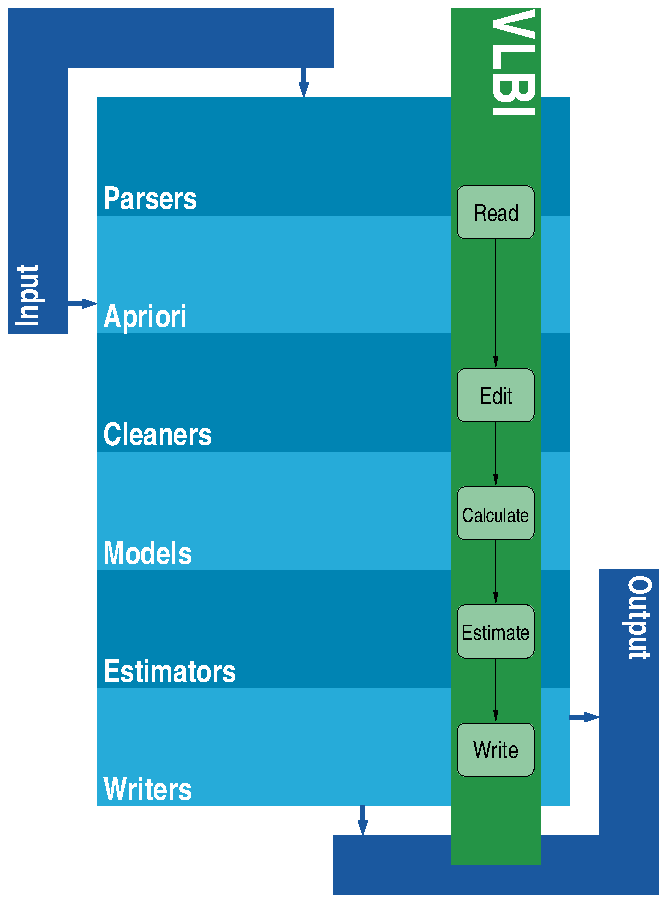
\includegraphics[width=.5\textwidth]{hjelle01.pdf}
  \caption{The VLBI pipeline. The stages \emph{Read}, \emph{Edit}, \emph{Calculate}, \emph{Estimate}, and \emph{Write} are performed sequentially to perform a VLBI analysis. Other pipelines can be defined that may reuse the common \where\ components: \emph{Parsers}, \emph{Apriori}, \emph{Cleaners}, \emph{Models}, \emph{Estimators}, and \emph{Writers}.}
  \label{fig:pipeline}
\end{figure}

Figure~\ref{fig:pipeline} illustrates the VLBI pipeline in green. Pipelines are based on a few simple principles:
\begin{itemize}
\item Stages in a pipeline are performed sequentially.
\item The output from one stage is input to the next stage.
\item The state of an analysis can be inspected at each stage.
\end{itemize}

While the pipelines are tailored to one particular kind of analysis, each stage rely on components that are common to all pipelines. This is illustrated as horizontal, blue boxes in Figure~\ref{fig:pipeline}.

This architecture makes it easy to reuse code across techniques. For instance, different pipelines can use the same ITRF component for a priori station positions, the same ocean loading model for station displacements or the same Kalman filter estimator.

\where\ comes bundled with a graphical tool for looking at and analyzing results from an analysis. This tool is called \there. Figure~\ref{fig:there} shows a screenshot of \there\ in action. More information about \there\ will be given in Section~\ref{sec:analysing_results} below.

\begin{figure}[htb!]
  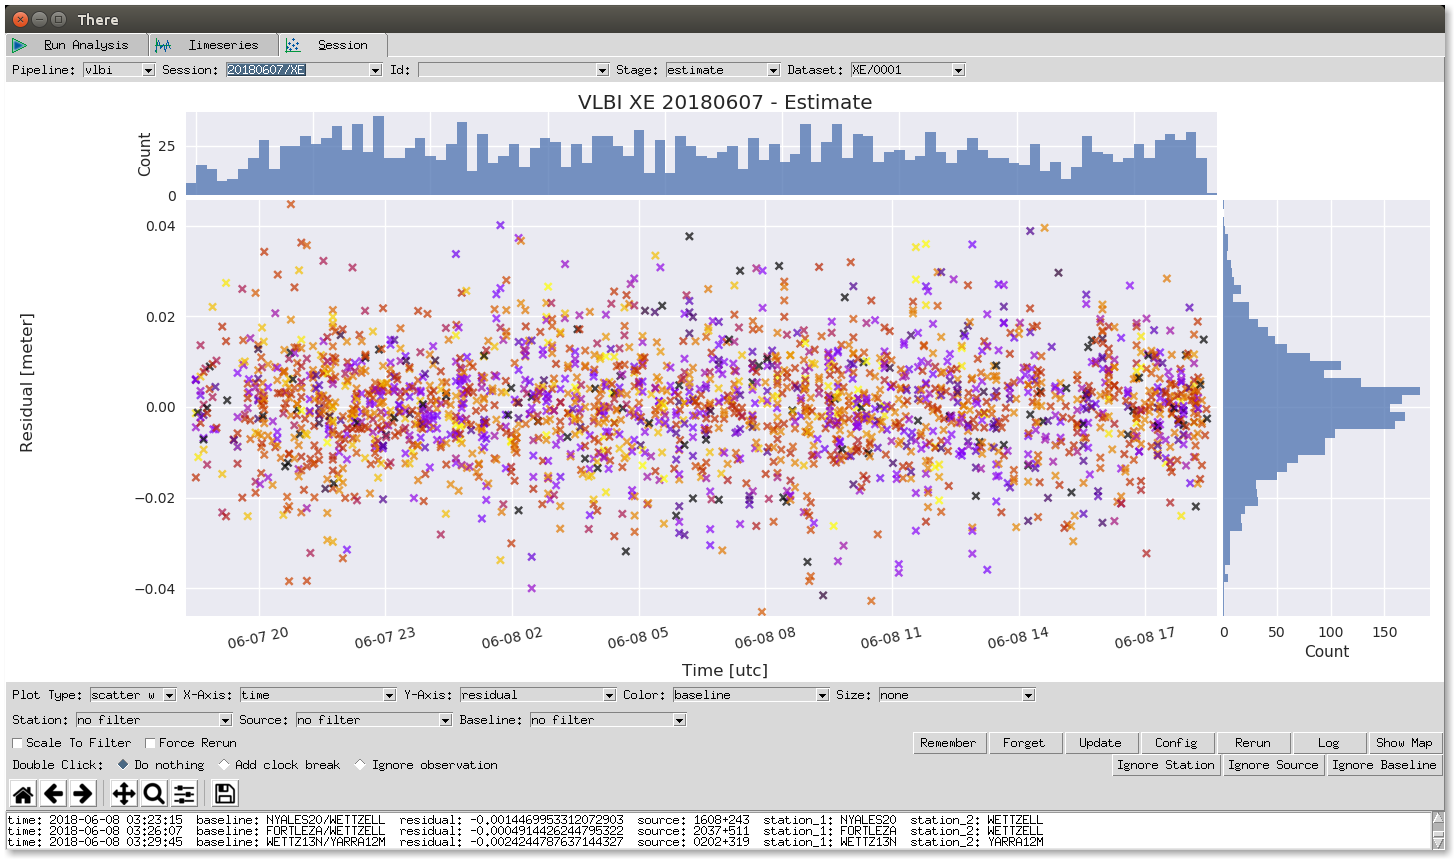
\includegraphics[width=.5\textwidth]{hjelle02.png}
  \caption{The \there\ graphical analysis tool. The plot shows post-fit residuals (after the \emph{Estimate} stage) for the XE session on June 7 2018. The colors indicate the baseline. That is, all residuals for the same baseline have the same color.}
  \label{fig:there}
\end{figure}

In an effort to make the functionality of \where\ as available as possible, components that can be reused outside \where\ pipelines are being separated into its own package called \midgard. While \midgard\ has its own web page\footnote{\url{kartverket.github.io/midgard/}}, it is most easily installed through the Python Package Index (PyPI)\footnote{\url{pypi.org/project/midgard/}} using the standard \textsf{Pip} tool:

\code{\$ pip install midgard}

Section~\ref{sec:midgard} contains more information.
%
\section{Try It Yourself}
%
\where\ is available through the GitHub platform. GitHub\footnote{\url{github.com}} is a place for sharing code and working together on software development. In addition to downloading \where\ and using it for your own analysis, you may also contribute to the further development of the software. Get in touch\footnote{\url{kartverket.github.io/where/pages/contact.html}} if you have any questions.

To start using \where\ you first need to install Python. We recommend the Anaconda Python distribution\footnote{\url{www.anaconda.com/download}}, as it bundles Python together with a lot of useful data science tools. Once you have Python on your system follow the instructions at the \where\ web page\footnote{\url{kartverket.github.io/where/installing.html}} to install the program.

Once the program is installed you can run an analysis. This is done with a command of the form

\code{\$ where 2018 6 7 --vlbi --session=XE}

The date, pipeline, and session must be specified. When executed, this will perform a VLBI analysis with the default settings (see Section~\ref{sec:configuration} below for more information). The program will automatically download all auxilliary files needed to do the analysis.

All information about an analysis, including the configuration, a list of file dependencies, and intermediate and final results are stored in a separate directory. While running the analysis, \where\ will by default print information about what it is doing to the console. The name of the analysis directory is printed at the top of this log, and the log is also stored to a file inside the analysis directory.
%
\section{Changing the Analysis Parameters}
\label{sec:configuration}
%
Most aspects of a \where\ analysis are configurable. The default configuration is defined in configuration files\footnote{\url{github.com/kartverket/where/tree/master/config}}. You can change the default configuration for all analyses by creating a file called \code{where\_local.conf} inside a directory called \code{.where} that resides in your home directory.

You can look at the configuration of an analysis by using the \code{where\_setup} tool:

{\footnotesize\begin{verbatim}
$ where_setup 2018 6 7 -v --session=XE
=======================================
VLBI XE 2018-06-07

[vlbi]
atmospheric_tides              = cm
atmospheric_tides_cmc          = False
ephemerides                    = de430
...
\end{verbatim}}

Individual parameters can be changed by specifying them on the command line when running either \code{where} or \code{where\_setup}:

{\footnotesize\begin{verbatim}
$ where 2018 6 7 -v --session=XE \
        --ephemerides=de421
\end{verbatim}}

You can also use the \code{-E} (\code{--edit}) option to open and change the configuration in an editor:

\code{\$ where 2018 6 7 -v --session=XE -E}

While NMA so far has used \where\ to analyse 24 hour R1 and R4 sessions, the software can analyse other kinds of VLBI sessions as well by changing the configuration appropriately. To easily work with different kind of sessions, \where\ supports configuration profiles. You can for example analyse the XU intensive session on June 7 2018 as follows:

{\footnotesize\begin{verbatim}
$ where 2018 6 7 -v --session=XU \
        --profile=intensives
\end{verbatim}}

A graphical utility for setting up and changing the configuration is in preparation. It will be integrated into \there\ later.
%
\section{Running Analyses}
\label{sec:analysing_results}
%
To run a series of analyses you can use the \code{where\_runner} tool. It will use master files\footnote{\url{ivscc.gsfc.nasa.gov/program/control\_files.html}} to call \where\ for all sessions in a specified time interval. For example, to analyse all sessions in January 2018 use the following:

\code{\$ where\_runner 2018 1 1 2018 1 31 --vlbi}

If you try to rerun an analysis you have already done, \where\ will by default do so in the same directory as before. \where\ is also lazy software, so it will not even do the analysis unless either the configuration or at least one of the input files have changed.

When comparing different models or settings you will be interested in running the same analysis twice and keeping the results. The way to do this is to label each of your analyses using the \code{--id} option:

{\footnotesize\begin{verbatim}
$ where 2018 6 7 -v --session=XE \
        --id=vtrf \
        --reference_frames=vtrf
\end{verbatim}}

The results from an analysis can be inspected using the \there\ graphical tool. Starting \there\ is usually done only by specifying that you want to look at VLBI analyses (either \code{-v} or \code{--vlbi}):

\code{\$ there -v}  

This opens the \there\ application. \there\ is organised using tabs. Along the top you will see different tabs including \emph{Timeseries} and \emph{Session}.

The \emph{Timeseries} is used to get an overview over all sessions that have been analysed. It can display many different summary parameters for each session, including residuals (see Figure~\ref{fig:there_timeseries}), size of session, and estimated parameters. Clicking on a point gives more information in the status bar at the bottom of the window.

\begin{figure}[t]
  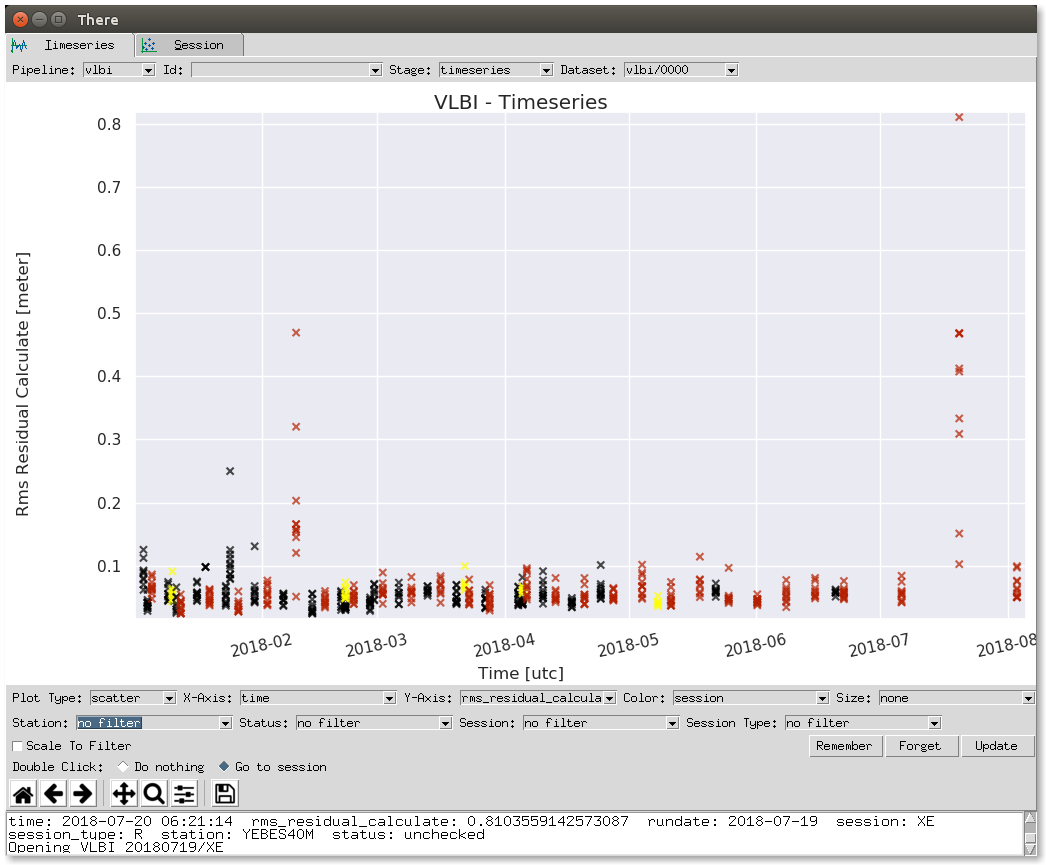
\includegraphics[width=.5\textwidth]{hjelle03.png}
  \caption{An overview over analysed sessions. The \emph{Timeseries} tab shows aggregated information about many sessions. In this example you can see that a few sessions (including one in July 2018) have much higher residuals than is normal. The colors indicate session name.}
  \label{fig:there_timeseries}
\end{figure}

You can also choose \emph{Go to session} and then double click on a point to investigate that session closer. This will open the \emph{Session} tab as in Figure~\ref{fig:there_session}.

The dropdown menus can be used to choose everything from plot type, to which variables to show, to filters that can be applied to the data. Each point represents one observation in the session. Clicking on a point shows information about that observation in the status bar.

You can edit a session from within \there. As an example, consider Figure~\ref{fig:there_session}. There is a clock break at around 13:00 UTC that should be edited out. \where\ has preliminary support for detecting clock breaks by itself. To mark the clock break and rerun the analysis, you do the following:

\begin{itemize}
\item Choose \emph{Add clock break}
\item Filter on the station in question, in this example YEBES40M
\item Double click in the plot where the clock break should be added. You might need to zoom in to do this precisely.
\item Click the \emph{Rerun} button
\end{itemize}

After rerunning the analysis, \there\ will update with the improved residuals.

Other editing operations like ignoring single observations or all observation for stations, baselines or sources are available directly in the \there\ interface. However, more complicated editing can be done by opening the configuration file. This is easiest done by clicking the \emph{Config} button.

\begin{figure}[t]
  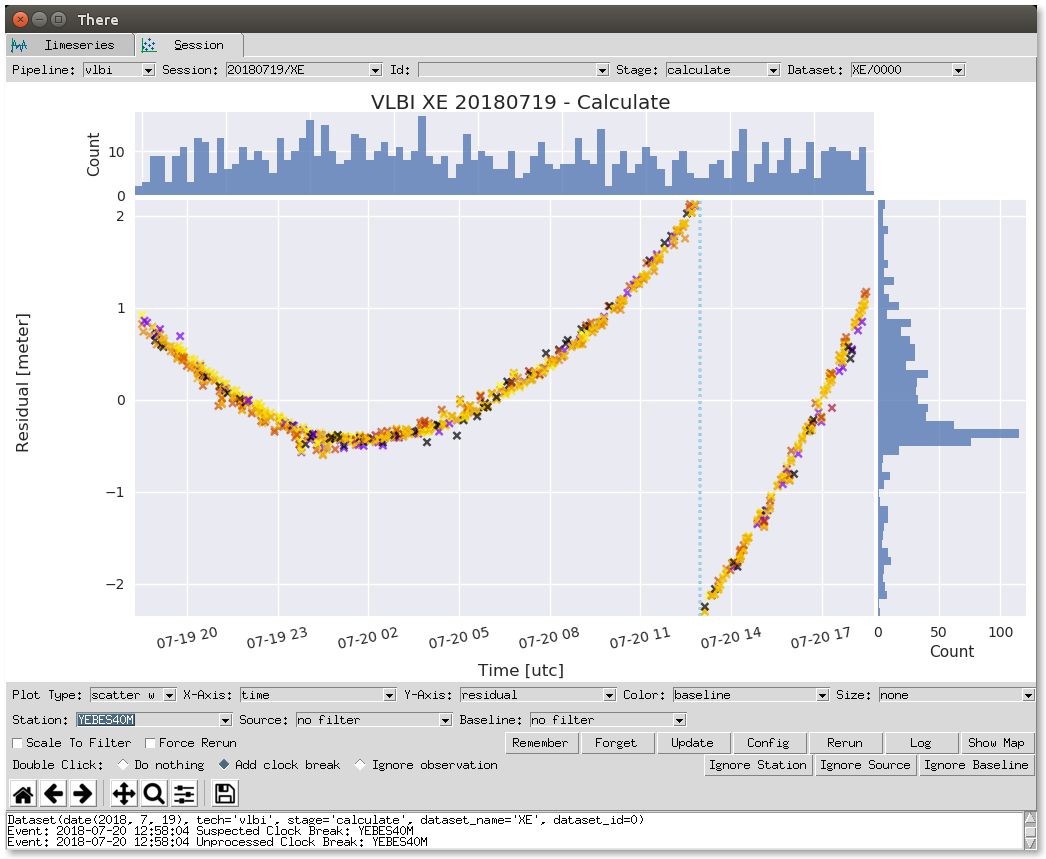
\includegraphics[width=.5\textwidth]{hjelle04.png}
  \caption{Looking at the results from one analysis. The \emph{Session} tab shows information about one particular session. The current plot shows prefit residuals for the XE session on July 19 2018. The results have been filtered to only show the YEBES40M station. A clock break is clearly visible in the residuals at around 13:00 UTC, and marked with a blue dashed line.}
  \label{fig:there_session}
\end{figure}

One other option for getting insight about the results of an analysis is to plot the results on a map. Clicking the \emph{Show Map} button in \there\ will open an interactive map in your browser. The map shows all stations and baselines in the session. Colors are used to show the size of the residuals (green is smaller), while the size of circles and width of lines represent the number of observations for a given station or baseline.

The map illustrates the geometry of the solution. As it is interactive you can also zoom and pan, and for instance look at local conditions at a site.
%
\section{Reuse in Your Own Programs}
\label{sec:midgard}
%
If you are using Python for programming geodetic applications or analysing geodetic data, \midgard\ might also be interesting to you directly.

\midgard\ is a library containing more general purpose geodetic functionality. \where\ uses \midgard\ extensively, and the plan is to move all parts of \where\ that can be reused to \midgard. Moving common components to \midgard\ is an ongoing process. Check the web page\footnote{\url{kartverket.github.io/midgard/}} for the current status.

You can use \midgard\ also if you are not using \where. In that case, first install \midgard\ using \code{pip}:

\code{\$ pip install midgard}

You can then use \midgard\ in your own scripts. For instance to read a Rinex file\footnote{\url{en.wikipedia.org/wiki/RINEX}} you can do something like:

{\footnotesize\begin{verbatim}
>>> from midgard import parsers
>>> path = "ALGO00CAN_R_20121601000.rnx"
>>> parsers.parse_file("rinex3_obs", path)
\end{verbatim}}

More information about \midgard\ and examples of how to use it is available online.

\begin{figure}[t]
  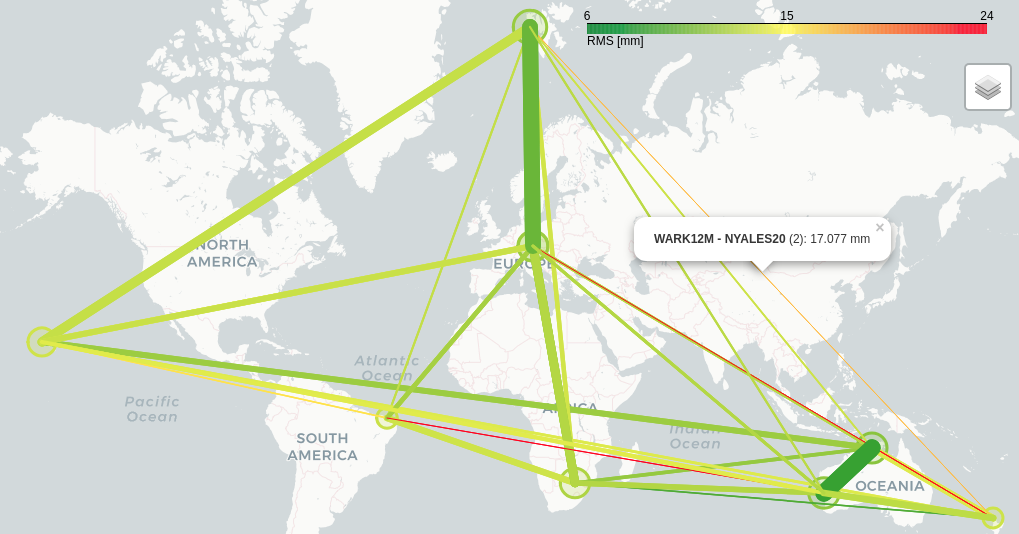
\includegraphics[width=.5\textwidth]{hjelle05.png}
  \caption{Interactive map of one analysis. The colors indicate the size of the residuals on given stations and baselines. The size of a circle and the width of a line show how many observations were used for a station or baseline, respectively}
  \label{fig:map}
\end{figure}
%
\section{Conclusions}
%
At the time of writing, the latest available version of \where\ is v0.12.1. However, new development on \where\ is ongoing, and we plan to release version 1.0.0 within 2018. See the web page\footnote{\url{kartverket.github.io/where/}} for the latest updates.

Please get in touch\footnote{\url{kartverket.github.io/where/pages/contact.html}} if you find \where\ useful or have any questions.
%
\begin{thebibliography}{99}

\bibitem{where_joss}
Hjelle, G.~A., et~al., Where: A scientific python package for geodetic
  analysis, in preparation.

\bibitem{kirkvik2017a}
Kirkvik, A.-S., Norwegian mapping authority analysis center {IVS} biennial
  report 2015--2016, in Baver, K.~D., Behrend, D., Armstrong, K.~L. (eds.),
  \emph{International VLBI Service for Geodesy and Astrometry 2015+2016
  Biennial Report}, 2017.

\bibitem{kirkvik2017b}
Kirkvik, A.-S., et~al., Where - a new software for geodetic analysis, in Haas,
  R., Elgered, G. (eds.), \emph{Proceedings of the 23rd European VLBI Group for
  Geodesy and Astrometry Working Meeting}, 2017.

\bibitem{kirkvik2018}
Kirkvik, A.-S., et~al., {NMA} analysis center -- progress report, IVS General
  Meeting Proceedings, IVS, 2018.

\end{thebibliography}
\end{document}
